\documentclass[english,11pt]{beamer}

\DeclareMathOperator{\Cov}{Cov}
\DeclareMathOperator{\Var}{Var}
\DeclareMathOperator{\E}{\mathbb{E}}
\DeclareMathOperator{\Proba}{\mathbb{P}}

\newcommand{\Covb}[2]{\ensuremath{\Cov\!\left[#1,#2\right]}}
\newcommand{\Eb}[1]{\ensuremath{\E\!\left[#1\right]}}
\newcommand{\Pb}[1]{\ensuremath{\Proba\!\left[#1\right]}}
\newcommand{\Varb}[1]{\ensuremath{\Var\!\left[#1\right]}}

% norm
\newcommand{\norm}[1]{\| #1 \|}

\newcommand{\indep}{\rotatebox[origin=c]{90}{$\models$}}





\usepackage{mathptmx,amsmath,amssymb,graphicx,bibentry,bbm,babel,ragged2e}

\makeatletter

\newcommand{\noun}[1]{\textsc{#1}}
\newcommand{\jitem}[1]{\item \begin{justify} #1 \end{justify} \vfill{}}
\newcommand{\sframe}[2]{\frame{\frametitle{#1} #2}}

\newenvironment{centercolumns}{\begin{columns}[c]}{\end{columns}}
%\newenvironment{jitem}{\begin{justify}\begin{itemize}}{\end{itemize}\end{justify}}

\usetheme{Warsaw}
\setbeamertemplate{footline}[text line]{}
\setbeamercolor{structure}{fg=purple!50!blue, bg=purple!50!blue}

\setbeamersize{text margin left=15pt,text margin right=15pt}

\setbeamercovered{transparent}


\@ifundefined{showcaptionsetup}{}{%
 \PassOptionsToPackage{caption=false}{subfig}}
\usepackage{subfig}

\usepackage[utf8]{inputenc}
\usepackage[T1]{fontenc}



\makeatother

\begin{document}


\title{Investigating the Empirical Existence of Static User Equilibrium}

\author{J.~Raimbault$^{1,2}$\\
\texttt{juste.raimbault@parisgeo.cnrs.fr}
}


\institute{$^{1}$UMR CNRS 8504 G{\'e}ographie-cit{\'e}s\\
$^{2}$UMR-T IFSTTAR 9403 LVMT\\
}


\date{EWGT 2016\\\smallskip
\textit{Session Transportation Modeling}\\\smallskip
5th September 2016
}

\frame{\maketitle}



%%%%%%%%%%%%%%%%%
\section{Introduction}
%%%%%%%%%%%%%%%%%



\sframe{Traffic Modeling : User Equilibrium Frameworks}{

\justify

% from static user eq to recent theoretical framework

\textit{Equilibrium frameworks central in Transportation Research since Wardrop \cite{wardrop1952road}}

\bigskip

Recent Developments :

\medskip

$\rightarrow$ Dynamic Stochastic User Equilibrium~\cite{han2003dynamic}

\medskip

$\rightarrow$ Restricted Stochastic User Equilibrium~\cite{rasmussen2015stochastic} more realistic in alternatives

\medskip

$\rightarrow$ Boundedly User Equilibrium~\cite{mahmassani1987boundedly}

\medskip

$\rightarrow$ Assignment techniques inspired from other fields such as Network Science~\cite{puzis2013augmented}

}


\sframe{Validation and Practical Use}{

% 

\textit{Static User Equilibrium lacks emirical validation in the literature}

Behavioral study of route choices in \cite{zhu2010people}

\cite{leurent2014user}


}


\sframe{Empirical Investigation of SUE Existence}{

\textbf{Research Objective : } \textit{Investigate empirically the spatio-temporal stationarity of flows, combining different quantitative approaches} 

}


%%%%%%%%%%%%%%%%%
\section{Results}
%%%%%%%%%%%%%%%%%



\sframe{Data Collection}{

\textit{Difficulty to find Open Data on Transportation Systems \cite{bouteiller2013open}}

$\rightarrow$ Construction of an open historical travel time dataset for major links in the region of Paris, collecting in real time public data from


}



\sframe{Interactive Data Visualization}{

\textit{Interactive web-application for spatio-temporal exploration}

\medskip


\includegraphics[width=\textwidth]{figures/gr1}

}



\sframe{Spatio-temporal Variability : Example}{

\textit{Very high spatial variability on 10min time interval}

\medskip

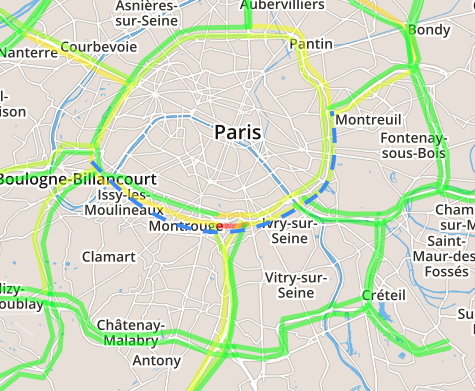
\includegraphics[width=0.47\textwidth]{figures/gr21}\hfill
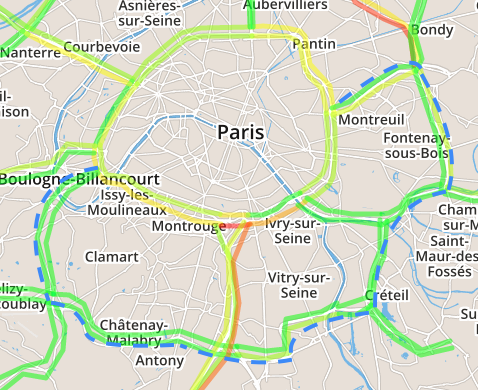
\includegraphics[width=0.47\textwidth]{figures/gr22}

}


\sframe{Spatio-temporal Variability}{

\textit{Maximal travel time and spatial variabilities}

\medskip

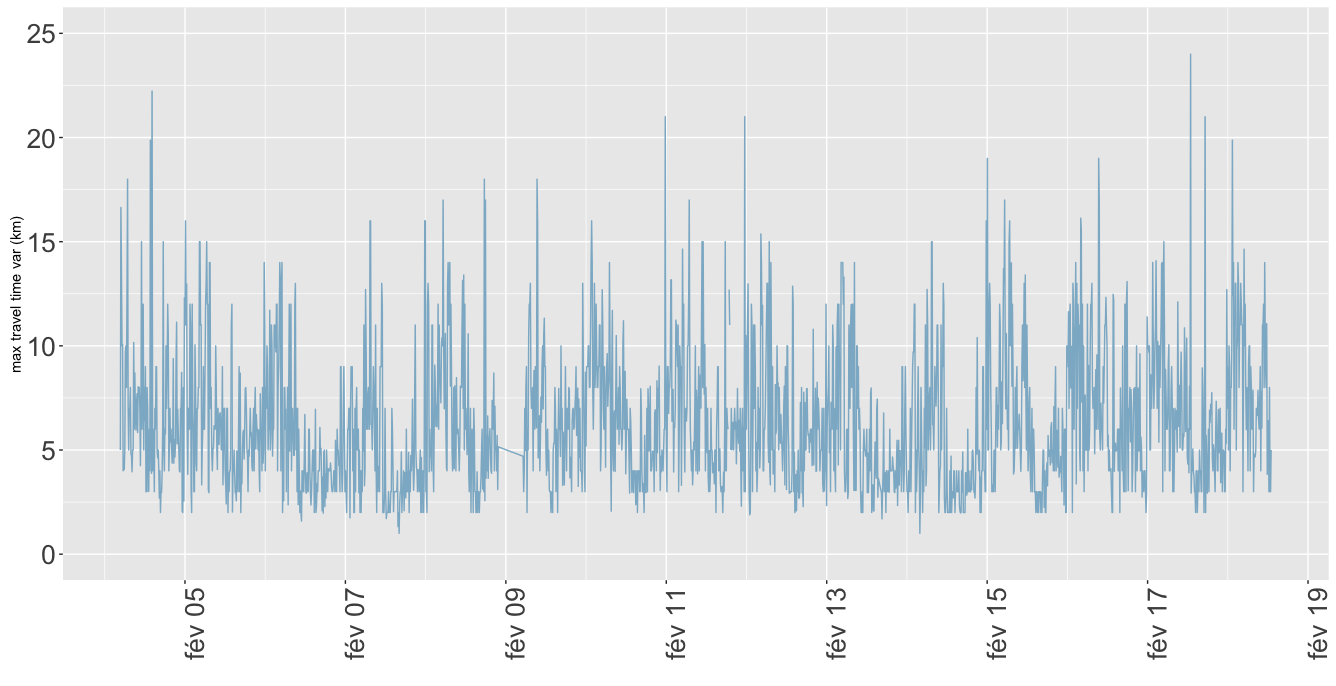
\includegraphics[width=0.5\textwidth]{figures/gr31}
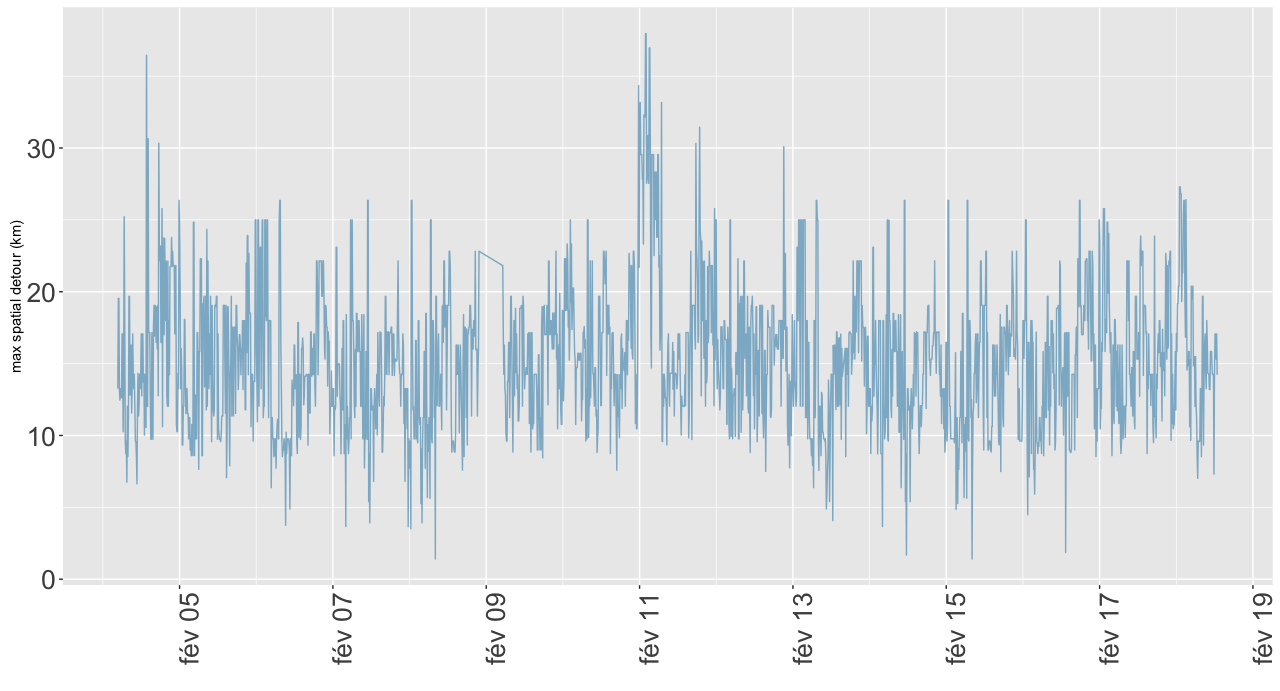
\includegraphics[width=0.5\textwidth]{figures/gr32}

}



\sframe{Stability of Network Measures}{

Network Betweenness Centrality 

\begin{equation}
b_i = \frac{1}{N(N-1)}\cdot \sum_{o\neq d \in V}\mathbbm{1}_{i\in p(o\rightarrow d)}
\end{equation}

Variability

\begin{equation}
\Delta b(t) = \frac{\left|\max_i (b_i(t + \Delta t)) - \max_i (b_i(t))\right|}{\max_i (b_i(t))}
\end{equation}

}


\sframe{Stability of Network Measures}{
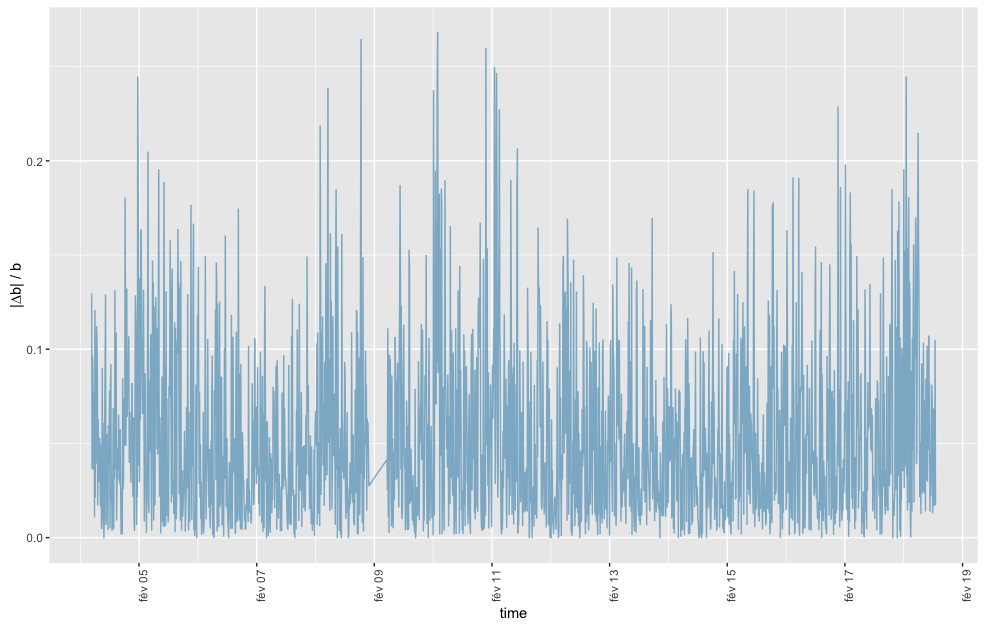
\includegraphics[width=\textwidth]{figures/gr4}
}



\sframe{Spatial Heterogeneity}{

Spatial Autocorrelation as an index of spatial variability

\begin{equation}
\rho_i = \frac{1}{K}\cdot \sum_{i\neq j}{w_{ij}\cdot (c_i - \bar{c})(c_j - \bar{c})}
\end{equation}

with weights  $w_{ij} = \exp{\left(\frac{-d_{ij}}{d_0}\right)}$

}



\sframe{Spatial Heterogeneity}{
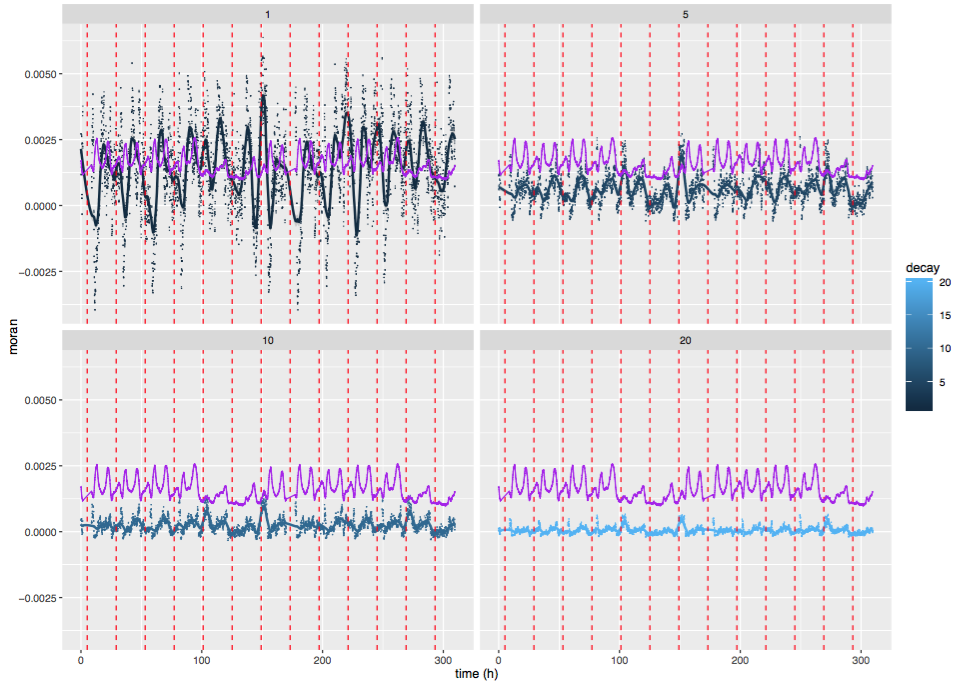
\includegraphics[width=\textwidth]{figures/moran_withCong}
}


%%%%%%%%%%%%%%%%%
\section{Discussion}
%%%%%%%%%%%%%%%%%


\sframe{Theoretical and Practical Implications}{

\textbf{Theoretical Implications}

$\rightarrow$ Need for more systematic comparison of framework validity : multi-modeling. \cite{kryvobokov2013comparison} compares two LUTI models

$\rightarrow$ Can still be used e.g. for integration within more complex models

\bigskip

\textbf{Practical Implications}

$\rightarrow$


}



\sframe{Explanative Interpretations}{


}


\sframe{Possible Developments}{


}



\sframe{Conclusion}{


}






%%%%%%%%%%%%%%%%%%%%%
\begin{frame}[allowframebreaks]
\frametitle{References}
\bibliographystyle{apalike}
\bibliography{/Users/Juste/Documents/ComplexSystems/CityNetwork/Biblio/Bibtex/CityNetwork,biblio}
\end{frame}
%%%%%%%%%%%%%%%%%%%%%%%%%%%%












\end{document}







